% ----------------------------------------------
% ----------------------------------------------
% \subsection{Traditional adversarial label \textbf{does not introduce label flipping noise}}
% \subsection{Traditional adversarial label does not introduce label noise directly}
\subsection{Label noise does not explicitly exist in the adversarially augmented training set}
\label{sect:label-flipping-noise}

\chengyu{Remove this section?}
% \sout{In standard learning, it is often necessary to manually inject label noise to make the double descent evident for modern neural architectures~\citep{Nakkiran2020DeepDD, Yang2020RethinkingBT}.}

% Since label noise is often essential to explain double descent in standard learning for modern neural architectures~\citep{Nakkiran2020DeepDD, Yang2020RethinkingBT},
% We wish to check if the traditional adversarial label produces any label flipping noise, a typical type of label noise, namely if $\tilde{y}_\delta \ne y^*_\delta$ for any adversarial example $x_\delta$.
% \chengyu{It is still possible there is a tiny fraction of label noise. But won't make a big difference.}
% the assigned label of the adversarial example is different from its true label.
% This is equivalent to checking if $ y^* \ne y_\delta^* $, since $\tilde{y}_\delta = y$ by the definition of the traditional adversarial label (Definition~\ref{remark:common-practice}) and $y = y^*$ by the property of our clean dataset (Assumption~\ref{assumption:clean-dataset}). Note that $y^* \ne y_\delta^*$ means the semantics of the adversarial example is distorted significantly such that its argmax label is now different from the argmax label of its clean counterpart. % , which is possible under adversarial perturbation.


    % The common practice in adversarial training assumes that an adversarial example shares the same true label with its clean counterpart, i.e., $\hat{y}_{\delta} \leftarrow \hat{y}$.
    % Since we have to pick one label for each instance and we have assumed $p(\hat{y} | x) = p(y | x)$, this assumption can be formally viewed as ``$\argmax_j ~p(y_{\delta}=j|x + \delta) = \argmax_j ~p(y=j|x)$''. 
    % Here, we show that this assumption does not introduce label flipping noise, which is often necessary to produce double descent in modern neural architectures in standard classifier training.


% \begin{figure*}[!ht]
% \centering
% % \begin{subfigure}{1.0\textwidth}
%   \centering
%   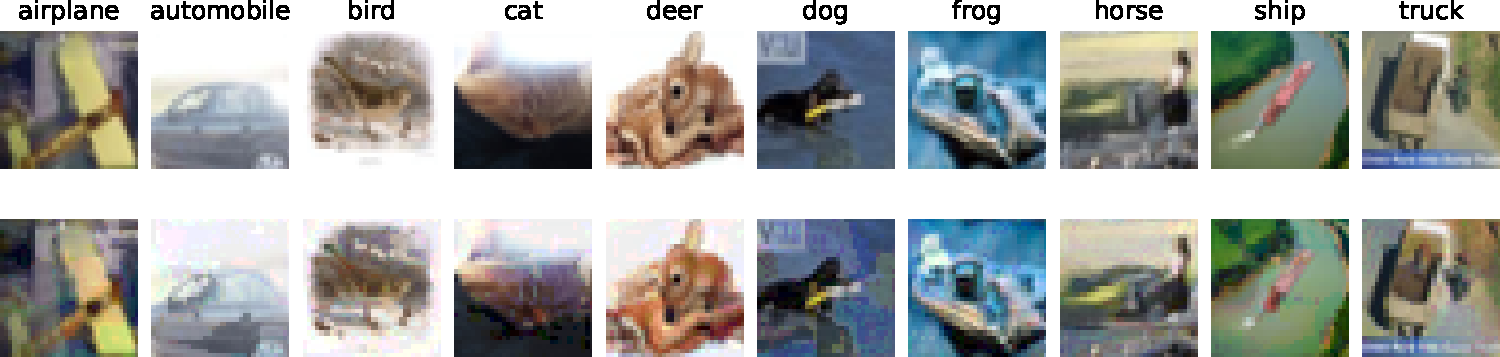
\includegraphics[width=0.95\linewidth]{figures/examples-low-quality.pdf}
%   % \caption{Examples with the lowest quality and their corresponding adversarial examples.}
%   % \label{fig:problematic-examples-orig}
% % \end{subfigure}
% % \begin{subfigure}{1.0\textwidth}
% %   \centering
% %   \includegraphics[width=0.95\linewidth]{figures/examples-high-quality.pdf}
% %   \caption{Examples with the highest quality and their corresponding adversarial examples.}
% %   \label{fig:problematic-examples-ad}
% % \end{subfigure}
%   \caption{Examples with the lowest and highest quality identified in the training set of CIFAR-10. In each subfigure, the top row shows the original image and the bottom row shows the image after the adversarial perturbation (PGD-10 with perturbation radius $8/255$). For each image, the true label is annotated on the top.}
%   % , and the predicted label is annotated on the bottom.}
% \label{fig:examples}
% \end{figure*}



We check if the adversarially augmented training set constructed from the benchmark dataset contains any noisy labels, namely the assigned labels that are different from their corresponding true labels.
    % We first visually check the adversarial examples created by the inner maximization in adversarial training. 
    We are specifically interested in those inputs with the lowest data quality as they are mostly likely to become label noise after perturbation.
    We estimate data quality based on model ensemble (see Appendix~\ref{sect:data-quality-estimation}).
    One can find that the adversarial examples of those low-quality inputs still match their original labels, albeit being slightly more ambiguous (see Figure~\ref{fig:illustration} and \todo{more samples in Appendix.}). 
    
    Evidence can also be found by charting the geometrical structure of the benchmark dataset.
    % \citet{Yang2020ACL} study the distance between examples in the input space. 
    In CIFAR-10 training set, \citet{Yang2020ACL} found that the minimum distance between any two inputs with different labels is around $50/255$ in terms of $\ell_\infty$ norm. In contrast, the perturbation radius used in adversarial training is typically $8/255$, which is significantly smaller. Therefore, it is unlikely that adversarial perturbation will change the true labels of the training inputs.
    It is thus reasonable to argue that label noise does not explicitly exist in the adversarially augmented training set in abundance.
    % Subsequently it cannot adequately explain the double descent observed in adversarial training.